%!TEX root = ../dissertation.tex
\chapter{Introduzione}
\label{ch:Introduzione}
In questo capitolo verrà introdotta l'azienda ospitante e le tecnologie da essa utilizzate.
\section{L'azienda}
Data Reply S.r.l fa parte delle aziende del gruppo Reply S.p.a e si occupa del mondo \emph{big data}, \emph{data science} e \emph{artificial intelligence}. L'azienda è giovane sia nella sua creazione, dato che è stata fondata nel 2013, sia dal punto di vista della composizione del personale. Questo le permette di avere flessibilità e freschezza mentale (in termini di idee) ma allo stesso tempo \emph{know how} e conoscenza del settore messa in campo dagli elementi con maggiore esperienza.

\begin{figure}
	\centering
	
\includegraphics[scale=2]{figures/data-reply-logo}
	\caption[Logo Data Reply S.r.l.]{Logo Data Reply S.r.l.
		\label{fig:logoDataReply}}
\end{figure}

Il mercato di Data Reply è quello della consulenza, un mondo spesso ostico e molto complesso ma che ha visto un'importante crescita degli investimenti in Italia negli ultimi anni.
\subsection{Le tecnologie da esplorare}
Le principali tecnologie utilizzate dall'azienda riguardano i settori \emph{big data}, \emph{Data Science} e \emph{Artificial Intelligence}. Troviamo un importante utilizzo delle suite di prodotti cloud, come Amazon Web Services (AWS) e Google Cloud, e di prodotti da poter utilizzare all'interno di macchine proprie, come \Gls{Cloudera}. Infine anche l'utilizzo di \emph{framework} per il calcolo distribuito, come Apache Spark, sono di fondamentale importanza.
\section{Processi del progetto}
\subsection{Metodologia di sviluppo}
All'interno di Data Reply vengono utilizzati diverse metodologie di sviluppo, che vanno dalle metodologie agile, nella quale vediamo tra le più utilizzate Scrum e Kanban, a metodologie a cascata. Essendo un'azienda di consulenza, spesso si trova a lavorare anche con altre aziende allo stesso progetto e per questo motivo non è raro trovare metodologie più rigide ai cambiamenti come le metodologie a cascata.
\subsection{Strumenti di supporto}
Gli strumenti di supporto utilizzati, come le metodologie di sviluppo,  sono decisi in base al progetto, al cliente e in accordo con le altre aziende che lavoreranno insieme al team Data Reply.
Di consueto, l'azienda propone l'utilizzo di Git come strumento di versionamento, GitLab per la gestione dei repository di lavoro e GitLab Mattermost per le comunicazioni informali tra i componenti del progetto e dell'azienda.
\subsection{Propensione alla modernizzazione}
L'azienda cerca sempre di rinnovarsi e rimanere al passo con le ultime tecnologie in modo da poter proporre ai propri clienti il giusto compromesso tra novità e affidabilità. Spesso infatti, vi sono progetti mirati allo studio ed utilizzo di tecnologie e prodotti da poco sul mercato, così da garantire un vantaggio competitivo sulle altre aziende.
Questo si può anche notare dai raduni svolti dall'azienda madre Reply nella quale Data Reply cerca sempre di portare progetti innovativi e che vadano a toccare le ultime tendenze del momento.
\section{La gestione dei dati}
I \emph{big data} hanno rivoluzionato le possibilità di utilizzo dei dati e con esso anche il modo in cui le aziende utilizzano i dati dei clienti e da loro prodotti. Per questo motivo, vi è sempre più attenzione sul come un dato viene trattato per essere immagazzinato e sfruttato al meglio.
\\
Nasce così il bisogno di acquisire dati in tempo reale o in \emph{batch}, conservarli e renderli accessibili in formato originale o anche in modi in cui le informazioni risaltino ancora di più all'occhio.
Questo processo viene chiamato \emph{\textbf{Data Ingestion}} ( o anche più semplicemente ingestion).
Questo, dunque, è solo una delle fasi che sono necessarie per la gestione dei dati.
Le altre possono essere riassunte in:
\begin{itemize}
	\item \emph{\textbf{Data Processing}}, nella quale troviamo la lavorazione del dato grezzo, in modo che sia pronto ad essere analizzato secondo gli standard aziendali e la capacità di automatizzare ed ingegnerizzare l'estrazione delle informazioni, in modo da rendere periodico e ripetibile il lavoro svolto sui dati;
	\item \emph{\textbf{Data Analysis}}, in cui viene svolta la ricerca e la creazione di modelli per l'estrazione di informazioni;
	\item \emph{\textbf{Data Integration}}, vi è la fruizione delle informazioni ricavate attraverso applicativi che interrogano i dati analizzati in modo da utilizzarli per scopi specifici (e.g. report aziendali).
\end{itemize}

\section{Cos'è l'anomaly detection?}
L'\emph{anomaly detection} è una tecnica statistica che permette di identificare "irregolarità" nei dati della serie temporale per un determinato valore di dimensione o metrica. 
Utilizzata sempre di più negli ultimi anni grazie alle nuove scoperte nel settore dei \emph{big data}, può rendere la vita di molti lavoratori più semplice notificando in modo repentino le situazioni che vanno al di fuori del normale.
\newpage
\begin{figure}[h!]
	\centering
	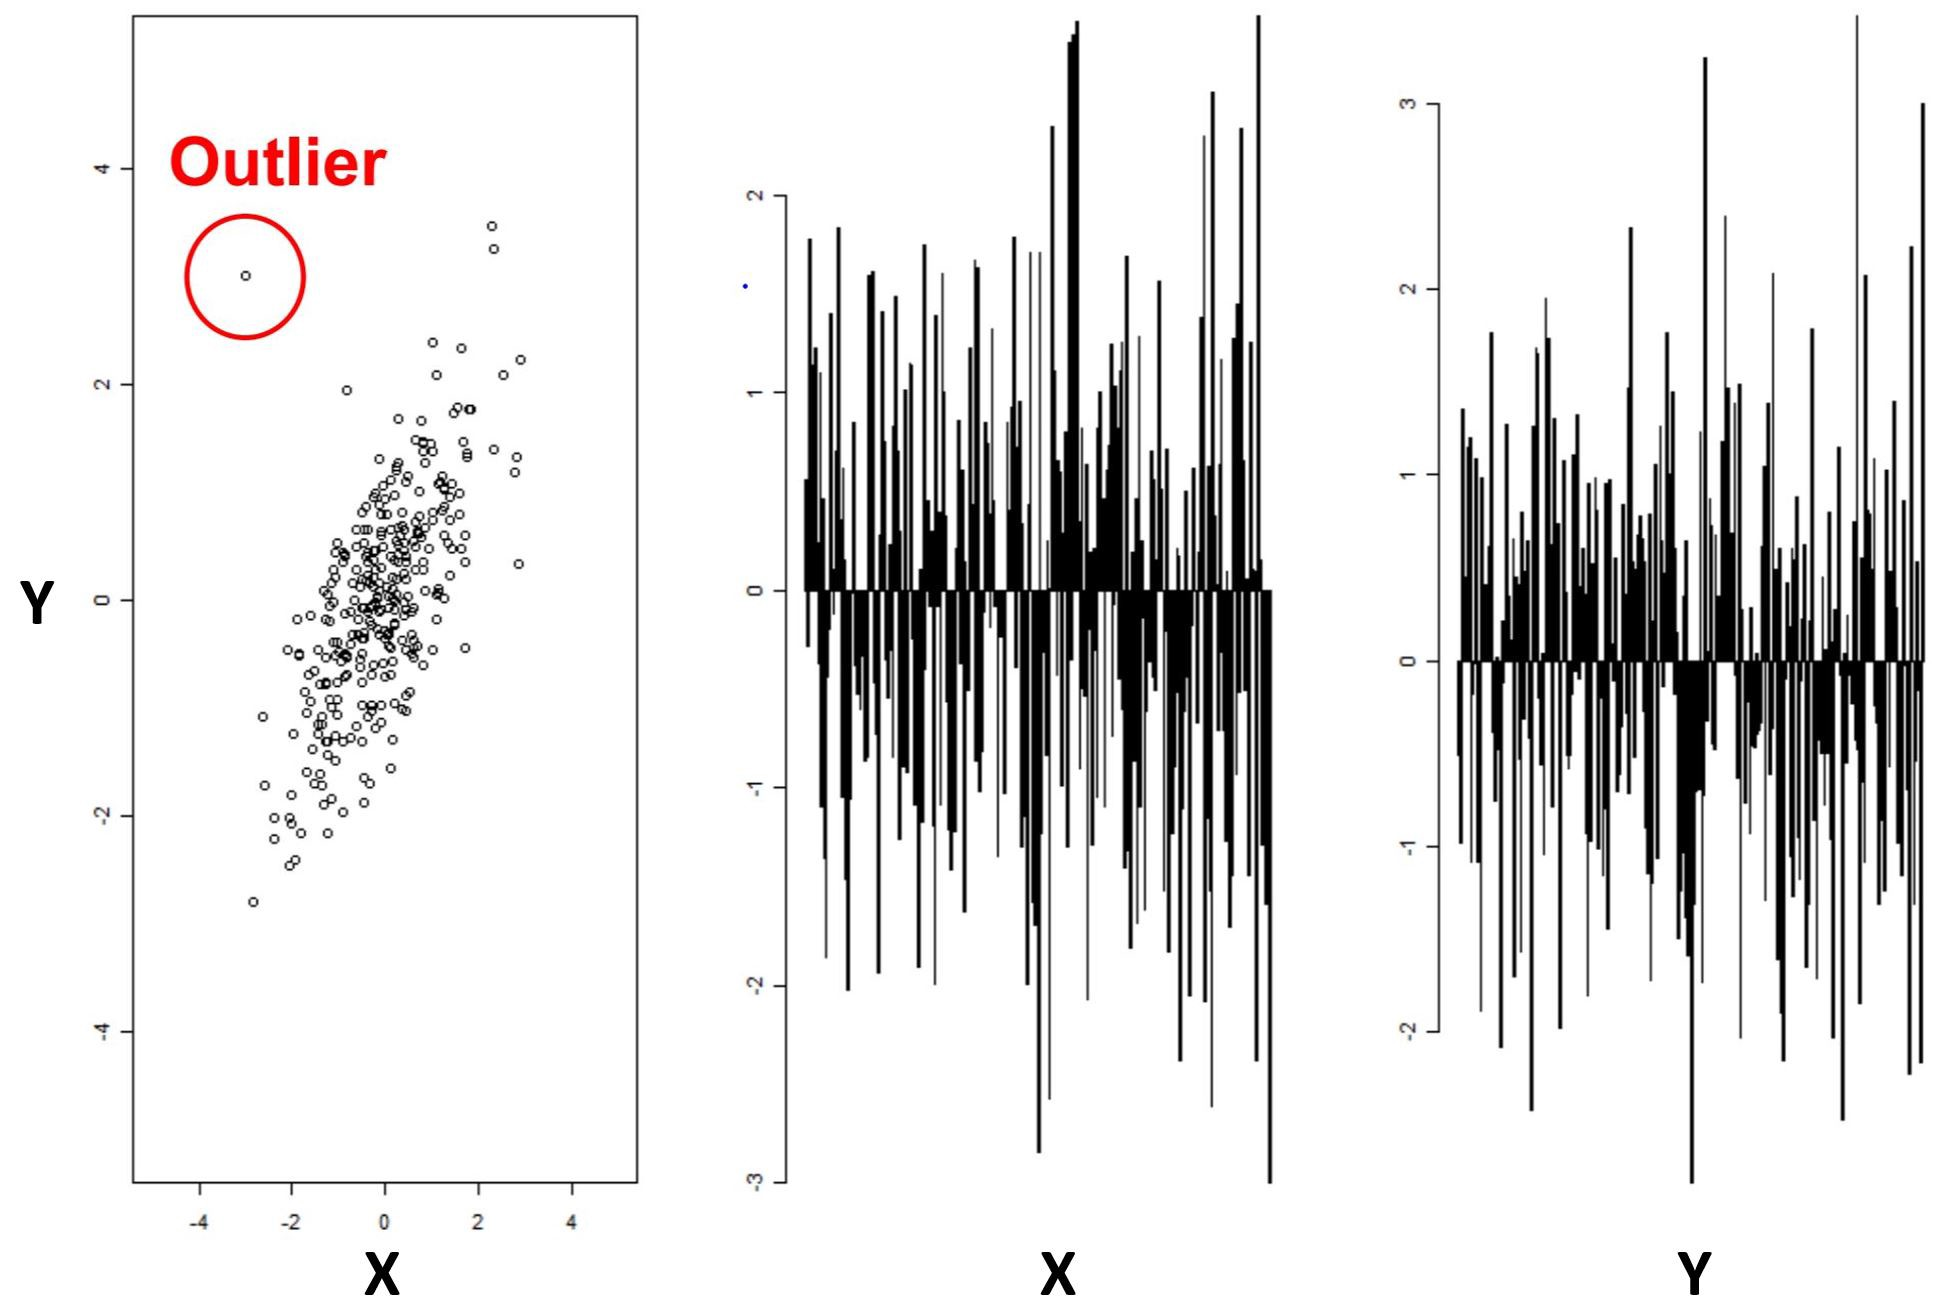
\includegraphics[scale=0.1]{figures/anomaly_detection_example}
	\caption[Esempio di anomalia.]{Esempio di anomalia \cite{anomalydetection}
		\label{fig:anomalia}}
\end{figure}	

Nell'immagine possiamo vedere un chiaro caso di anomalia, il punto cerchiato in rosso si trova al di fuori della normale distribuzione dei punti.
Il rilevamento delle anomalie risulta utile in molti settori, tra cui quello delle frodi bancarie e il monitoraggio dello stato del sistema. 
\section{Organizzazione del documento}
In questa sezione vengono riassunti i contenuti di ogni capitolo e le convenzioni tipografiche adottate.
\subsection{Contenuti}
\begin{description}
	\item[{\hyperref[ch:evoluzione-dello-stage]{Il secondo capitolo}}] descrive l'evoluzione dello stage, dalla proposta alla pianificazione del lavoro.
	
	\item[{\hyperref[ch:analisi-e-progettazione]{Il terzo capitolo}}] approfondisce l'analisi e la progettazione del progetto, descrivendo metodologia di lavoro, i requisiti trovati e i risultati ottenuti.
	
	\item[{\hyperref[ch:sviluppo]{Il quarto capitolo}}] approfondisce le tecnologie e gli strumenti affrontate spiegando l'integrazione fra tutte le parti.
	
	\item[{\hyperref[ch:conlusione]{Il quinto capitolo}}] vengono tratte le conclusioni e argomentate le considerazioni personali.
\end{description}
\subsection{Convenzioni tipografiche}
Riguardo la stesura del testo, relativamente al documento sono state adottate le seguenti convenzioni tipografiche:
\begin{itemize}
	\item gli acronimi, le abbreviazioni e i termini ambigui o di uso non comune menzionati vengono definiti nel glossario, situato alla fine del presente documento;
	\item i termini in lingua straniera o facenti parti del gergo tecnico sono evidenziati con il carattere \emph{corsivo}.
\end{itemize}
